\documentclass[serif, xcolor=dvipsnames]{beamer}

\makeatletter

%%%%%%%%%%%%%%%%%%%%%%%%%%%%%% User specified LaTeX commands.
%HAY QUE ELEGIR EL QUE CORRESPONDA

%\usepackage{mathpazo}%Letra palatino con fuentes para matemáticas
\usepackage[T1]{fontenc}
\usepackage[utf8]{inputenc}
\usepackage{graphicx}
\usepackage{url}
\usepackage{amsmath}
\usepackage{booktabs}
\usepackage{textcomp}%%needed for the euro symbol

\date{}

\usepackage[emulate=units]{siunitx}
\sisetup{per=fraction, fraction=nice, decimalsymbol=comma}
\newunit{\wattpeak}{Wp}
\newunit{\watthour}{Wh}
\newunit{\amperehour}{Ah}

\setbeamercovered{transparent}
\setbeamertemplate{navigation symbols}{}
\usefonttheme{structuresmallcapsserif} 
\usefonttheme{serif} 
\usefonttheme{structurebold}

%\usepackage{epstopdf}


\usepackage[spanish]{babel}
\addto\shorthandsspanish{\spanishdeactivate{~<>}}

\hypersetup{pdfauthor={Oscar Perpi\~n\'an},%
    pdftitle={Energ\'ia Solar Fotovoltaica},%
    filecolor=blue,%
    urlcolor=blue}



%\usepackage{handoutWithNotes} %para hacer papel con notas 
%\pgfpagesuselayout{4 on 1 with notes}[a4paper,border shrink=5mm]



%\usepackage{pgfpages}
%\pgfpagesuselayout{2 on 1}[a4paper,border shrink=5mm]


%\usepackage{mathpazo}%Letra palatino con fuentes para matemáticas
\usepackage[T1]{fontenc}
\usepackage[utf8]{inputenc}
\usepackage{graphicx}
\usepackage{url}
\usepackage{amsmath}
\usepackage{booktabs}

\usepackage[spanish]{babel}
\addto\shorthandsspanish{\spanishdeactivate{~<>}}


\usepackage{hyperref}
% \hypersetup{pdfauthor={Oscar Perpi\~n\'an},%
%     pdftitle={Energ\'ia Solar Fotovoltaica},%
%     filecolor=blue,%
%     urlcolor=blue}

\hypersetup{
    bookmarks=true,         % show bookmarks bar?
%    unicode=true,          % non-Latin characters in Acrobat’s bookmarks
    bookmarksnumbered=false,
    bookmarksopen=false,
    breaklinks=true,
    backref=true,
    pdftoolbar=true,        % show Acrobat’s toolbar?
    pdfmenubar=true,        % show Acrobat’s menu?
    pdffitwindow=false,     % window fit to page when opened
    pdfstartview={FitH},    % fits the width of the page to the window
    pdftitle={Energía Solar Fotovoltaica},    % title
    pdfauthor={Oscar Perpiñán Lamigueiro},     % author
    pdfsubject={Electrotecnia},   % subject of the document
    pdfcreator={AucTeX/Emacs},   % creator of the document
    pdfproducer={LaTeX}, % producer of the document
    pdfnewwindow=true,      % links in new window
    pdfborder={0 0 0},
    colorlinks=true,       % false: boxed links; true: colored links
    linkcolor=,          % color of internal links
    citecolor=BrickRed,        % color of links to bibliography
    filecolor=black,      % color of file links
    urlcolor=Blue           % color of external links 
}

\usepackage[emulate=units]{siunitx}
\sisetup{per=fraction, fraction=nice, decimalsymbol=comma}
\newunit{\wattpeak}{Wp}
\newunit{\watthour}{Wh}
\newunit{\amperehour}{Ah}

\setbeamercovered{transparent}
\setbeamertemplate{navigation symbols}{}
\usefonttheme{serif} 
\usefonttheme{structuresmallcapsserif} 

\useinnertheme[shadow=true]{rounded}
\useoutertheme{shadow}
%\usecolortheme[named=BrickRed]{structure} %sirve para cambiar el color genérico
\usecolortheme{orchid}
\usecolortheme{whale}
\documentclass[xcolor={usenames,svgnames,dvipsnames}]{beamer}
\usepackage[utf8]{inputenc}
\usepackage[T1]{fontenc}
\usepackage{graphicx}
\usepackage{grffile}
\usepackage{longtable}
\usepackage{wrapfig}
\usepackage{rotating}
\usepackage[normalem]{ulem}
\usepackage{amsmath}
\usepackage{textcomp}
\usepackage{amssymb}
\usepackage{capt-of}
\usepackage{hyperref}
\usepackage{color}
\usepackage{listings}
\usepackage{mathpazo}
\usepackage{gensymb}
\usepackage{amsmath}
\usepackage{chemarr}%flechas para reacciones químicas (SFER.tex)
\bibliographystyle{plain}
\AtBeginSubsection[]{\begin{frame}[plain]\tableofcontents[currentsubsection,sectionstyle=show/shaded,subsectionstyle=show/shaded/hide]\end{frame}}
\AtBeginSection[]{\begin{frame}[plain]\tableofcontents[currentsection,hideallsubsections]\end{frame}}
\usepackage[emulate=units]{siunitx}
\sisetup{fraction=nice, decimalsymbol=comma, retain-unity-mantissa = false}
\newunit{\wattpeak}{Wp}
\newunit{\watthour}{Wh}
\newunit{\amperehour}{Ah}
\usepackage{steinmetz}
\hypersetup{colorlinks=true, linkcolor=OliveGreen, urlcolor=Blue}
\renewcommand{\thefootnote}{\fnsymbol{footnote}}
\beamertemplatenavigationsymbolsempty
\setbeamertemplate{footline}[frame number]

\setbeamercolor{alerted text}{fg=Green!50!black} \setbeamerfont{alerted text}{series=\bfseries}
\usefonttheme{serif}
\setbeamercovered{transparent}
\setbeamertemplate{navigation symbols}{}
\usefonttheme{serif} 

\setbeamercolor{palette primary}{bg=OliveGreen,fg=white}
\setbeamercolor{palette secondary}{bg=OliveGreen,fg=white}
\setbeamercolor{palette tertiary}{bg=OliveGreen,fg=white}
\setbeamercolor{palette quaternary}{bg=OliveGreen,fg=white}
\setbeamercolor{structure}{fg=OliveGreen} % itemize, enumerate, etc
\setbeamercolor{section in toc}{fg=OliveGreen} % TOC sections

\usetheme[hideothersubsections]{Goettingen}

\usepackage{tikz}

\titlegraphic{
\includegraphics[width=2.5cm]{../figs/logoEOI.jpg}}
\addtobeamertemplate{frametitle}{}{%
\begin{tikzpicture}[remember picture,overlay]
\node[anchor=south east,yshift=2pt] at (current page.south east) {
\includegraphics[width=1.5cm]{../figs/logoEOI.jpg}};
\end{tikzpicture}}


\makeatother

\begin{document}

\title{\textsc{Energía Solar Fotovoltaica:}\\
\textsc{Radiación Solar}}

\date{}

\author{\textsc{Oscar Perpiñán Lamigueiro}}

\begin{frame}[plain]
  \titlepage
\end{frame}

\AtBeginSection[]{
    \begin{frame}
        \frametitle{Índice}
        \tableofcontents[currentsection] 
    \end{frame} 

                  }

\selectlanguage{spanish}%

\section{Estadística}


\begin{frame}
\frametitle{Variable aleatoria y proceso estocástico}
\begin{itemize}
\item Una variable aleatoria es una función que asigna un único numero real
a cada resultado de un espacio muestral en un experimento.
\item Un proceso estocástico es una variable aleatoria que evoluciona a
lo largo del tiempo (p.ej. la radiación). 
\end{itemize}

\end{frame}
\begin{frame}
\frametitle{Función de densidad de probabilidad}

La función de densidad de probabilidad, $f(X)$, de una variable aleatoria
asigna probabilidad a un suceso:\[
P(a<X<b)=\int_{a}^{b}f(x)dx\]


\[
P(X<b)=\int_{-\infty}^{b}f(x)dx\]


\[
P(X>a)=\int_{a}^{\infty}f(x)dx\]



\end{frame}

\begin{frame}[plain]
\frametitle{Función de Densidad de Probabilidad}

\begin{center}
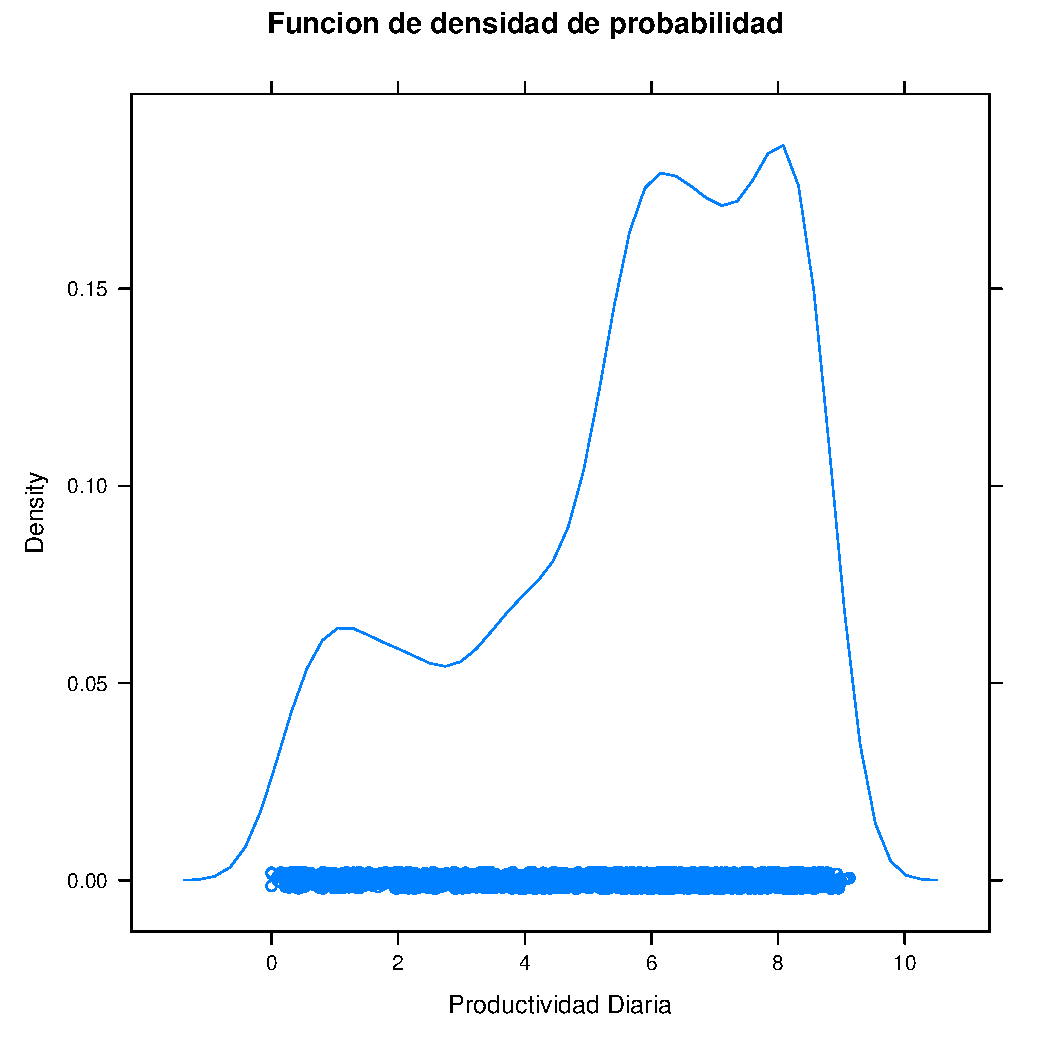
\includegraphics[scale=0.45]{../Figuras/FuncionDensidadProbabilidad}
\par\end{center}


\end{frame}

\begin{frame}[plain]
\frametitle{Histograma}

\begin{center}
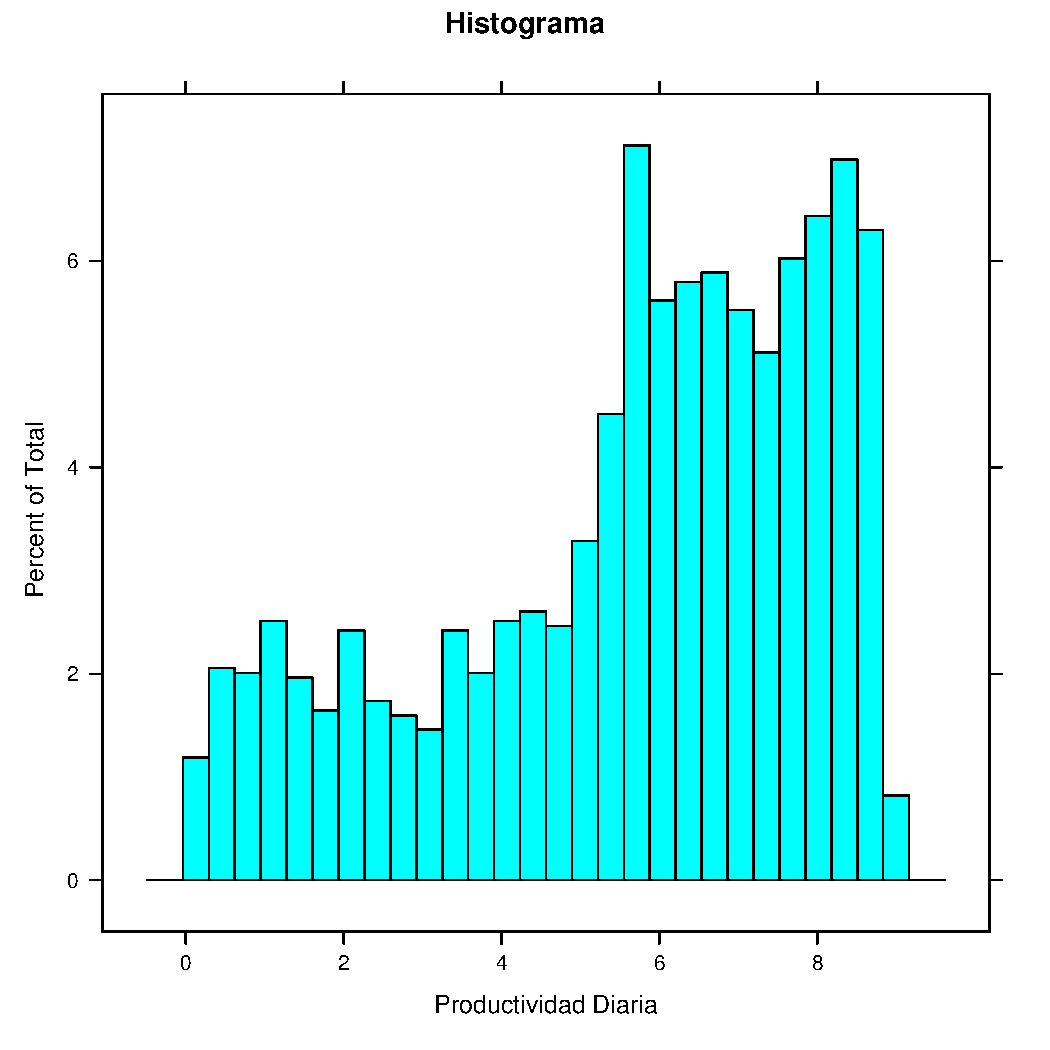
\includegraphics[scale=0.45]{../Figuras/Histograma}
\par\end{center}


\end{frame}
\begin{frame}
\frametitle{Media, varianza y desviación estándar}

La media de una variable aleatoria es el centro de masas de su función
densidad de probabilidad:\[
\mu_{X}=\int_{-\infty}^{\infty}x\cdot f(x)dx\]


La varianza de una variable aleatoria es la media del cuadrado de
las desviaciones respecto a la media:\[
\sigma_{X}^{2}=\int_{-\infty}^{\infty}(x-\mu_{X})^{2}\cdot f(x)dx\]


La desviación estándar es la raiz cuadrada de la varianza: $\sigma_{X}=\sqrt{\sigma_{X}^2}$


\end{frame}
\begin{frame}
\frametitle{Combinación lineal de variables aleatorias}

La media de la suma de varias variables aleatorias independientes
es la suma de las medias:\[
\mu_{X_{1}+...+X_{n}}=\mu_{X_{1}}+...+\mu_{X_{n}}\]


La varianza de la \emph{suma o resta} de varias variables aleatorias
independientes es la \emph{suma} de las varianzas:\[
\sigma_{X_{1}\pm...\pm X_{n}}^{2}=\sigma_{X_{1}}^{2}+...+\sigma_{X_{n}}^{2}\]



\end{frame}
\begin{frame}
\frametitle{Media y varianza de la media muestral}

Una muestra de una población es un conjunto de variables aleatorias
independientes ($X_{1}...X_{n}$). Si se toma una muestra de una población
cuya media es $\mu$ y su varianza es $\sigma^{2}$, entonces la media
de la muestra es otra variable aleatoria:\[
\overline{X}=\frac{1}{n}\sum_{n}X_{i}\]


que es una suma de variables aleatorias. 


\end{frame}
\begin{frame}
\frametitle{Media y varianza de la media muestral}

Por tanto, la media de la media muestral es la suma de las medias:
\[
\overline{X}=\mu\]


y la varianza de la media muestral es la suma de las varianzas:\[
\sigma_{\overline{X}}^{2}=\sigma_{\frac{1}{n}X_{1}}^{2}+...+\sigma_{\frac{1}{n}X_{n}}^{2}=\frac{\sigma^2}{N}\]


Por tanto, una forma de reducir la incertidumbre es realizar la medida
en repetidas ocasiones.


\end{frame}
\begin{frame}
\frametitle{Mediana y cuartiles}
\begin{itemize}
\item La mediana divide el conjunto de valores de la variable en dos mitades
iguales (divide el area encerrada por la función densidad de probabilidad
en dos partes iguales).
\item Los cuartiles dividen este area en cuatro partes iguales. 
\item El area encerrada entre cada par de cuartiles es igual al 25\% del
total. 
\item La mediana es el segundo cuartil. 
\item La distancia intercuartil (definida entre los cuartiles 1 y 3) es
una medida de la dispersión de la variable.
\end{itemize}

\end{frame}

\begin{frame}[plain]
\frametitle{Gráficos boxplot}

\begin{center}
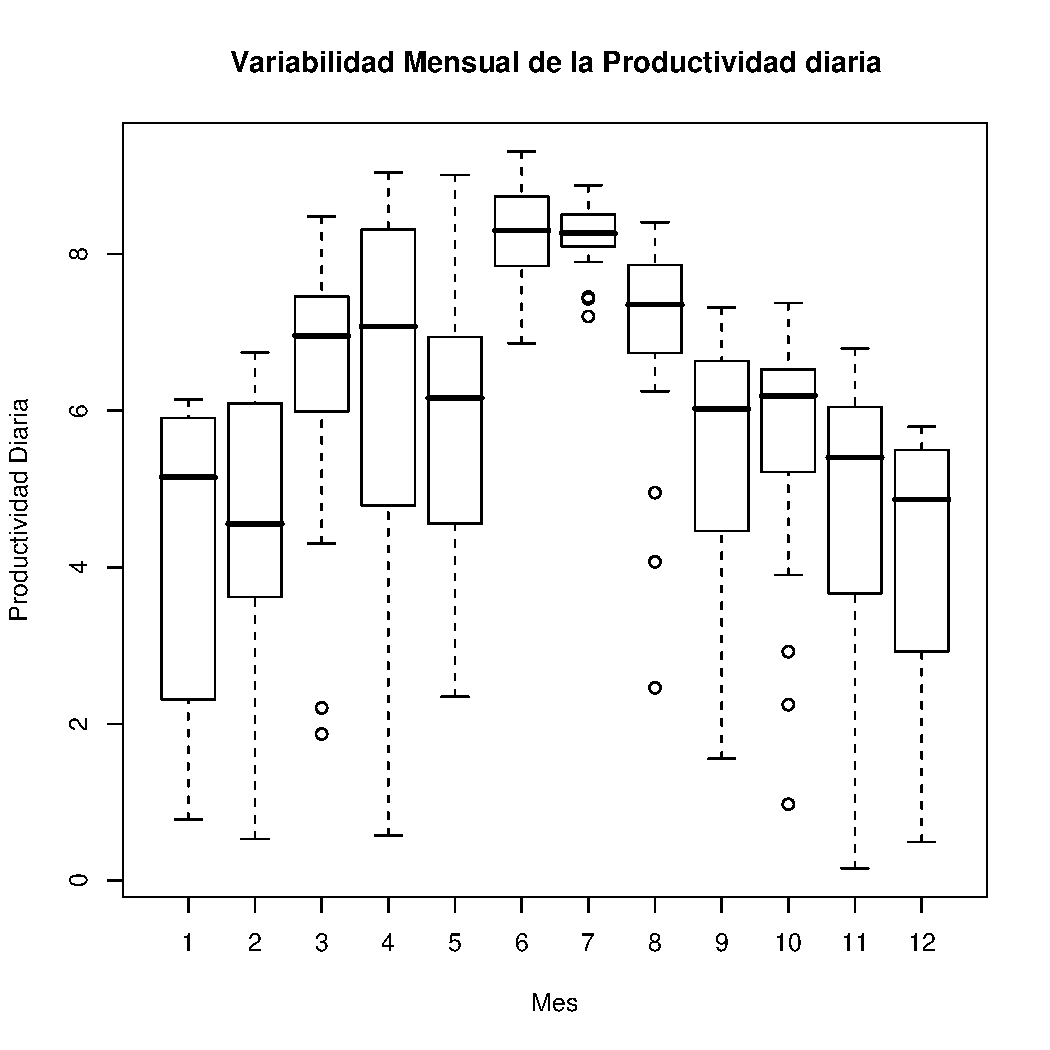
\includegraphics[scale=0.45]{../Figuras/GraficoBoxplot}
\par\end{center}


\end{frame}
\begin{frame}
\frametitle{Desviación entre modelo y observación}

Si tenemos un modelo que aproxima el comportamiento de una variable
aleatoria, definimos el error cuadrático medio como:\[
RMSE^{2}=\int_{-\infty}^{\infty}x^2_{D}\cdot f_{X_{D}}(x)dx=\sigma^2_{X_{D}}+\mu_{X_{D}}^{2}\]


siendo $X_{D}$ la variable aleatoria que define la desviación entre
modelo y observación. 

El coeficiente de correlación entre dos conjuntos de datos es una
medida numérica de la relación \emph{lineal }entre los dos conjuntos
(si la relación no es lineal, este coeficiente no sirve):\[
r=\frac{1}{n-1}\cdot\sum_{i=1}^{n}\left(\frac{x_{i}-\bar{x}}{\sigma_{X}}\right)\cdot\left(\frac{y_{i}-\bar{y}}{\sigma_{Y}}\right)\]



\end{frame}

\begin{frame}[plain]
\frametitle{Gráficos de dispersión}

\begin{center}
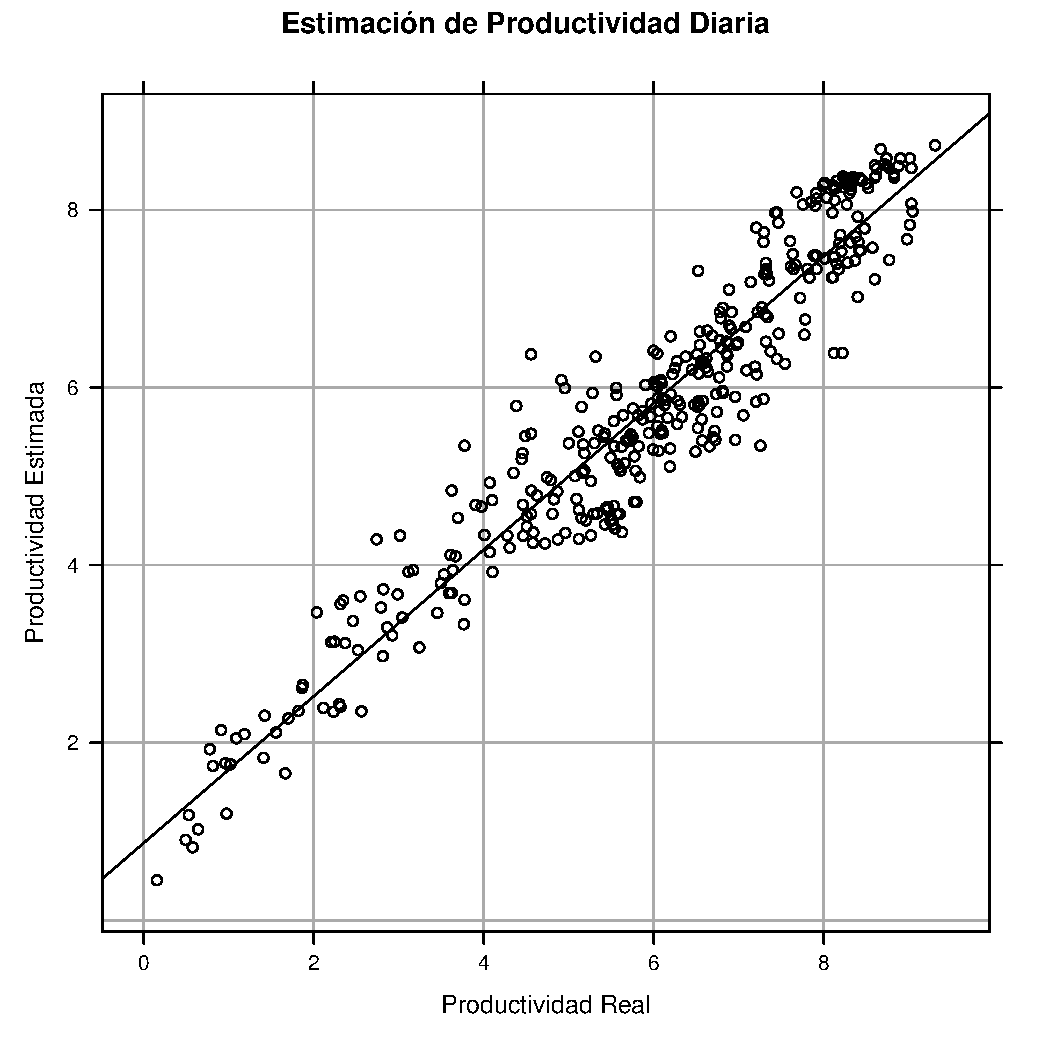
\includegraphics[scale=0.45]{../Figuras/GraficoDispersion}
\par\end{center}


\end{frame}

\section{Naturaleza de la radiación solar}


\begin{frame}
\frametitle{Irradiancia e Irradiación}
\begin{description}
\item [{Irradiancia}] es la densidad de \emph{potencia} de radiacion solar
incidente en una superficie. Unidades $\si{\watt\per\meter\squared},\,\si{\kilo\watt\per\meter\squared}$
\item [{Irradiación}] es la densidad de \emph{energía} de radiación solar
incidente en una superficie. Unidades: $\si{\watthour\per\meter\squared},\,\si{\kilo\watthour\per\meter\squared}$
\end{description}

\end{frame}
\begin{frame}
\frametitle{Radiación Extra-atmosférica}
\begin{itemize}
\item La radiación que alcanza la superficie de la atmósfera es radiación
directa del Sol.
\item \textbf{Constante solar} $B_{0}=\SI{1367}{\watt\per\meter\squared}$
(irradiancia solar sobre la superficie normal al vector solar en límite
superior de la atmósfera terrestre)
\item \textbf{Irradiancia extra-atmosférica}

\begin{itemize}
\item $B_{0}(0)=B_{0}\cdot\epsilon_{0}\cdot\cos\theta_{zs}$
\item $B_{0d}(0)=-\frac{T}{\pi}B_{0}\epsilon_{0}\cdot\left(\omega_{s}\sin\phi\sin\delta+\cos\delta\cos\phi\sin\omega_{s}\right)$\\
($\omega_{s}$ en radianes)
\end{itemize}
\end{itemize}

\end{frame}
\begin{frame}
\frametitle{Radiación Extra-atmosférica}
\begin{itemize}
\item Es posible demostrar que el \textbf{promedio mensual} de esta irradiación
diaria \textbf{coincide numericamente} con el valor de irradiación
diaria correspondiente a los denominados \textbf{{}``días promedios''},
días en los que la declinación correspondiente coincide con el promedio
mensual 
\item Por tanto, podemos calcular el valor medio mensual de la irradiación
diaria extra-atmosférica con el valor de la declinación de uno de
los doce días promedio.
\end{itemize}
\begin{center}
{\footnotesize }\begin{tabular}{>{\centering}p{6mm}>{\centering}m{4mm}>{\centering}m{4mm}>{\centering}m{4mm}>{\centering}m{4mm}>{\centering}m{4mm}>{\centering}m{4mm}>{\centering}m{4mm}>{\centering}m{4mm}>{\centering}m{4mm}>{\centering}m{4mm}>{\centering}m{4mm}>{\centering}m{3mm}}
\toprule 
{\footnotesize Mes} & {\footnotesize Ene} & {\footnotesize Feb} & {\footnotesize Mar} & {\footnotesize Abr} & {\footnotesize May} & {\footnotesize Jun} & {\footnotesize Jul} & {\footnotesize Ago} & {\footnotesize Sep} & {\footnotesize Oct} & {\footnotesize Nov} & {\footnotesize Dic}\tabularnewline
\midrule
$d_{n}$ & {\footnotesize 17} & {\footnotesize 45} & {\footnotesize 74} & {\footnotesize 105} & {\footnotesize 135} & {\footnotesize 161} & {\footnotesize 199} & {\footnotesize 230} & {\footnotesize 261} & {\footnotesize 292} & {\footnotesize 322} & {\footnotesize 347}\tabularnewline
\bottomrule
\end{tabular}
\par\end{center}{\footnotesize \par}


\end{frame}

\begin{frame}
\frametitle{Interacción de la radiación con la atmósfera}
\begin{itemize}
\item \textbf{Disminución} de la radiación incidente en la superficie terrestre
(reflexión en nubes)
\item \textbf{Modificación de las características espectrales} de la radiación
(absorción por vapor de agua, ozono y CO2)
\item \textbf{Modificación de la distribución espacial} (dispersión por
partículas)

\begin{itemize}
\item Difusión de Rayleigh (longitud de onda mucho mayor que tamaño de partícula)
- Capas altas - Color Azul
\item Difusión de Mie (longitud de onda de magnitud similar a tamaño de
partícula) - Capas bajas
\item Difusión no selectiva (longitud de onda mucho menor que tamaño de
partícula)
\end{itemize}
\end{itemize}

\end{frame}
\begin{frame}
\frametitle{Componentes de la radiación solar}
\begin{itemize}
\item \textbf{Radiación Directa}. (B)

\begin{itemize}
\item Linea recta con el Sol.
\end{itemize}
\item \textbf{Radiación Difusa}. (D)

\begin{itemize}
\item Procedente de todo el cielo salvo el Sol
\item Rayos dispersados por la atmósfera. 
\item Anisotrópica, proceso estocástico.
\end{itemize}
\item \textbf{Radiación del albedo}. (R, AL)

\begin{itemize}
\item Procedente del suelo (reflejada)
\end{itemize}
\item \textbf{Radiación Global:} $G=B+D+R$
\end{itemize}

\end{frame}
\begin{frame}
\frametitle{Cómo se escribe}


\framesubtitle{Forma, tiempo, lugar}
\begin{description}
\item [{Forma+Tiempo+Lugar:}] Irradiancia directa (forma) horaria (tiempo)
en el plano del generador (lugar)
\item [{Promedios:}] Media mensual (periodo) de la irradiación global (forma)
diaria (tiempo) 
\item [{Lugar:}]~


(Orientación, Inclinación) 

(0=Horizontal)

(n=Normal)

(I=Plano del generador)

\end{description}

\end{frame}
\begin{frame}
\frametitle{Cómo se escribe}


\framesubtitle{Forma, tiempo, lugar}

\[
Forma_{tiempo,promedio}(lugar)\]


\[
G_{d,m}(0),\, D_{h}(\alpha,\beta),\, B_{0d}(n),\, B(\beta)\]



\end{frame}
\begin{frame}
\frametitle{Caracterización de la atmósfera}
\begin{itemize}
\item \textbf{Masa de aire}: 

\begin{itemize}
\item Relación entre camino recorrido por rayos directos del Sol a través
de la atmósfera hasta la superficie receptora y el que recorrerían
en caso de incidencia vertical (AM=1)
\item $AM=1/\cos\theta_{zs}$
\end{itemize}
\item \textbf{Índice de claridad}

\begin{itemize}
\item Relación entre la radiación global en el plano horizontal y la radiación
extra-atmosférica en el plano horizontal
\item El índice de claridad \textbf{no depende de las variaciones debidas
al movimiento aparente del sol}.
\item $K_{Tm}=\frac{G_{d,m}(0)}{B_{0d,m}(0)}$ (mensual)
\end{itemize}
\end{itemize}

\end{frame}
\begin{frame}
\frametitle{Índice de claridad}
\begin{description}
\item [{$K_{T}$:}] índice de claridad instantáneo. $K_{T}=G/B_{0}$
\item [{$K_{Td}$:}] índice de claridad diario. $K_{Td}=G_{d}/B_{0d}$
\item [{$K_{Tm}$:}] índice de claridad mensual. $K_{Tm}=G_{m}/B_{0m}=G_{d,m}/B_{0d,m}$
\item [{$K_{Ta}$:}] índice de claridad anual. $K_{Ta}=G_{a}/B_{0a}=...$
\end{description}

\end{frame}
\section{Cálculo de componentes de radiación solar}


\begin{frame}
\frametitle{Radiación como proceso estocástico}
\begin{itemize}
\item La \textbf{distribución de valores} que presenta la radiación solar
durante un periodo está \textbf{determinada por el valor promedio
de la radiación durante ese periodo}. Por ejemplo, conocer la media
mensual de la radiación solar diaria en un determinado lugar permite
saber cómo se comportará la radiación diaria durante ese mes 
\item El índice de claridad para un día concreto \textbf{sólo está influido}
por el índice de claridad del \textbf{día anterior}. 
\end{itemize}

\end{frame}
\begin{frame}
\frametitle{Estimación de Directa y Difusa}
\begin{itemize}
\item Establecer una \textbf{relación entre la fracción difusa} de la radiación
horizontal ($F_{D}=\frac{D(0)}{G(0)}$) y \textbf{el índice de claridad}.
\item \textbf{Correlación negativa} (a mayor índice de claridad, menor componente
difusa)
\item \textbf{Correlación independiente de la latitud} (validez cuasi-universal)
\end{itemize}

\end{frame}

\begin{frame}[plain]
\frametitle{Correlaciones $F_{D}$ y $K_{T}$}


\framesubtitle{Ecuación de Page (medias mensuales) }

\[
F_{Dm}=1-1.13\cdot K_{Tm}\]


\begin{center}
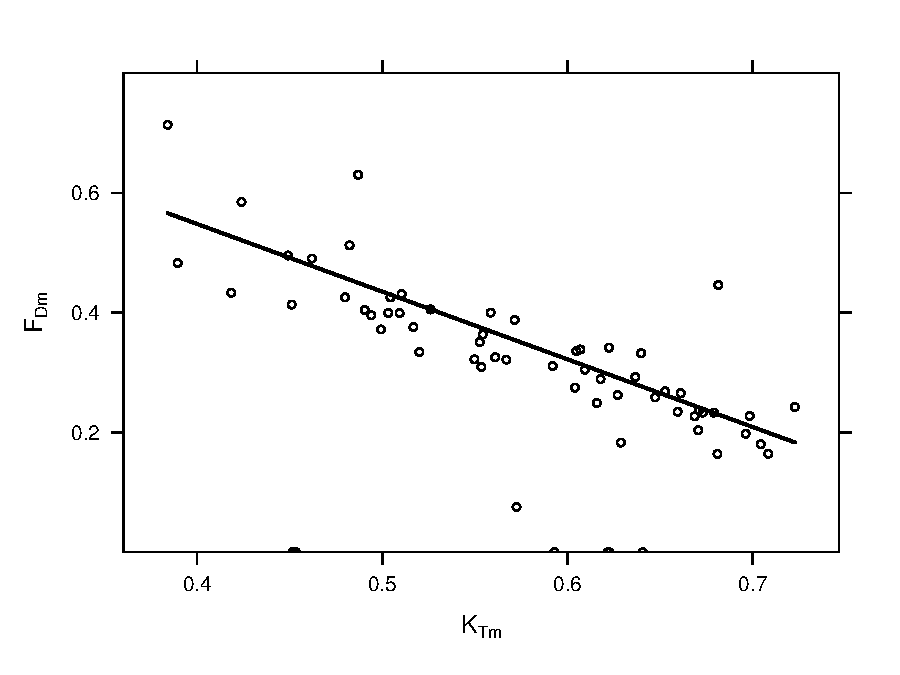
\includegraphics[scale=0.6]{../Figuras/FdKtMensual}
\par\end{center}


\end{frame}
\begin{frame}
\frametitle{Correlaciones $F_{D}$ y $K_{T}$}

Por ejemplo, un lugar que recibe en el plano horizontal $\SI{3150}{\watthour\per\meter\squared}$
de media mensual de irradiación global diaria en un mes que corresponde
a media mensual de irradiación extraterrestre diaria de $\SI{4320}{\watthour\per\meter\squared}$
tendrá, en ese mes, un índice de claridad mensual $K_{Tm}=\frac{3150}{4320}=0.73$ 

Según la correlación de Page, una fracción de difusa $F_{Dm}=1-1.13\cdot0.73=0.175$. 

La media mensual de radiación difusa diaria será $D_{d,m}(0)=0.175\cdot3150=\SI{551.6}{\watthour\per\meter\squared}$. 

La radiación directa en el plano horizontal será $B_{d,m}(0)=3150-551.6=\SI{2598,4}{\watthour\per\meter\squared}$.


\end{frame}

\begin{frame}[plain]
\frametitle{Correlaciones $F_{D}$ y $K_{T}$}


\framesubtitle{Ecuación de Collares-Pereira y Rabl (valores diarios)}

{\scriptsize \[
F_{Dd}=\begin{cases}
0.99 & K_{Td}\leq0.17\\
1.188-2.272\cdot K_{Td}+9.473\cdot K_{Td}^{2}-21.856\cdot K_{Td}^{3}+14.648\cdot K_{Td}^{4} & K_{Td}>0.17\end{cases}\]
}{\scriptsize \par}

\begin{center}
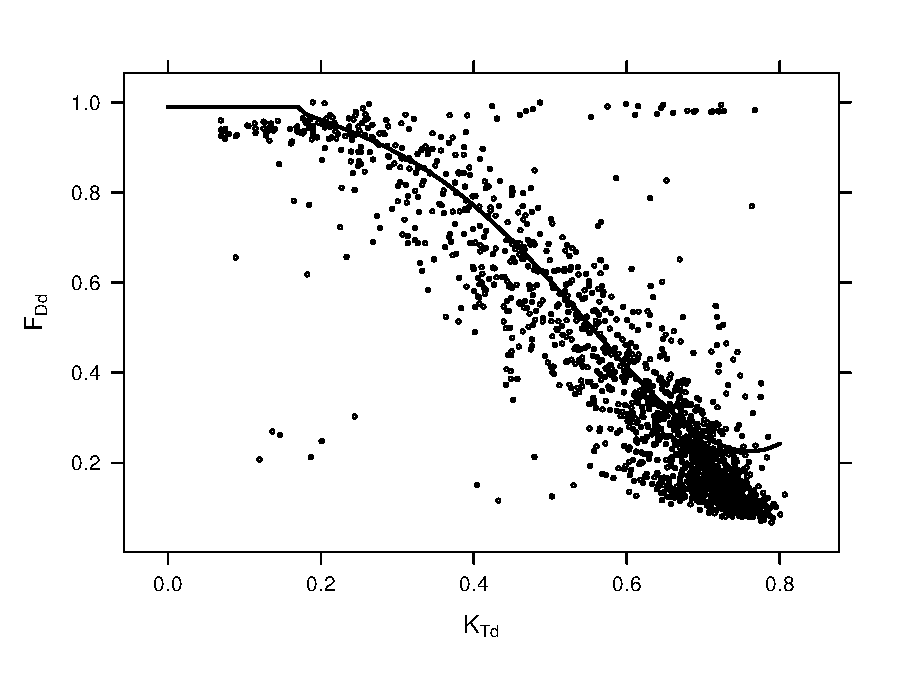
\includegraphics[scale=0.6]{../Figuras/FdKtDiario}
\par\end{center}


\end{frame}
\begin{frame}
\frametitle{Estimación de Directa y Difusa}
\begin{description}
\item [{Calcular}] las componentes directa y difusa de la radiación solar
del:

\begin{description}
\item [{Mes}] de Septiembre (día 261) en un lugar con latitud $\phi=\ang{40}\mathrm{N}$
y con media mensual de irradiación global diaria horizontal $G_{d,m}(0)=\SI{2700}{\watthour\per\meter\squared}$.
\end{description}
\end{description}

\end{frame}
\begin{frame}
\frametitle{Datos de radiación}
\begin{itemize}
\item Medidas procedentes de \textbf{estaciones meteorológicas}

\begin{itemize}
\item Piranómetro: Radiación Global
\item Pirheliómetro: Radiación Directa
\end{itemize}
\item Estimaciones basadas en \textbf{imágenes de satélite}
\end{itemize}

\end{frame}
\begin{frame}
\frametitle{Datos de radiación}


\framesubtitle{Estaciones Terrestres (selección)}
\begin{itemize}
\item Red SIAR:
  \url{http://eportal.magrama.gob.es/websiar/Inicio.aspx}
\item Xunta de Galicia:
  \url{http://www2.meteogalicia.es/galego/observacion/estacions/estacions.asp}
\item Castilla - La Mancha:
  \url{http://crea.uclm.es/siar/datmeteo/}
\item Navarra:
  \url{http://meteo.navarra.es/estaciones/mapadeestaciones.cfm}
\item Cataluña: \url{http://www.meteo.cat/xema/AppJava/SeleccioPerComarca.do}
\item NREL-MIDC: \url{http://www.nrel.gov/midc/}
\item HELIOS-IES (Madrid): \url{http://helios.ies-def.upm.es/}
\end{itemize}

\end{frame}
\begin{frame}
\frametitle{Datos de radiación}


\framesubtitle{Imágenes de satélite}
\begin{itemize}
\item EUMETSAT Satellite Application Facility on Climate Monitoring
  \url{http://www.cmsaf.eu}
\item NASA: \url{http://eosweb.larc.nasa.gov/cgi-bin/sse/grid.cgi?} 
\item PVGIS: \url{http://re.jrc.ec.europa.eu/pvgis/apps4/pvest.php} 
\item SODA-Esra: \url{http://www.soda-is.com/eng/services/services_radiation_free_eng.php}
\end{itemize}

\end{frame}
\section{Cálculo de radiación sobre generadores}



\begin{frame}[plain]
\frametitle{Irradiancia sobre superficies arbitrarias}

\begin{center}
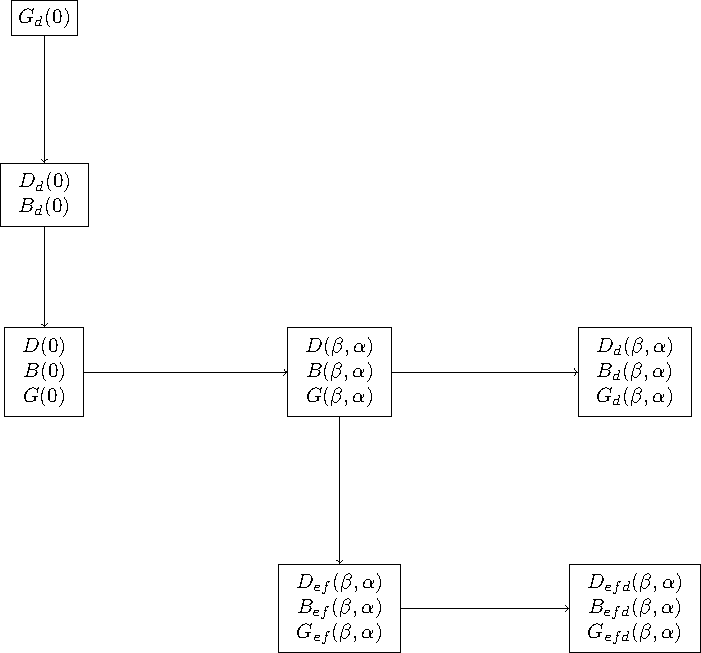
\includegraphics{../Figuras/ProcedimientoCalculoRadiacionInclinada}
\par\end{center}


\end{frame}

\subsection{Irradiancia a partir de irradiación diaria}


\begin{frame}
\frametitle{Estimación de Irradiancia a partir de Irradiación diaria}
\begin{itemize}
\item Irradiación durante una hora coincide con el valor medio de la irradiancia
durante esa hora.
\item Variación solar durante una hora es baja: valor de irradiancia equivalente
a valor de irradiación.
\item Relación entre irradiancia e irradiación extra-terrestre deducible
teóricamente:
\end{itemize}
\[
\frac{B_{o}(0)}{B_{0d}(0)}=\frac{\pi}{T}\cdot\frac{\cos(\omega)-\cos(\omega_{s})}{\omega_{s}\cdot\cos(\omega_{s})-\sin(\omega_{s})}\]



\end{frame}
\begin{frame}
\frametitle{Estimación de Irradiancia a partir de Irradiación diaria}
\begin{block}
{}

\[
r_{D}=\frac{D(0)}{D_{d}(0)}=\frac{B_{o}(0)}{B_{0d}(0)}\]


\[
r_{G}=\frac{G(0)}{G_{d}(0)}=r_{D}\cdot\left(a+b\cdot\cos(\omega)\right)\]


\[
a=0.409-0.5016\cdot\sin(\omega_{s}+\frac{\pi}{3})\]


\[
b=0.6609+0.4767\cdot\sin(\omega_{s}+\frac{\pi}{3})\]


\end{block}

\end{frame}

\begin{frame}[plain]
\frametitle{Estimación de Irradiancia a partir de Irradiación diaria}

\begin{center}
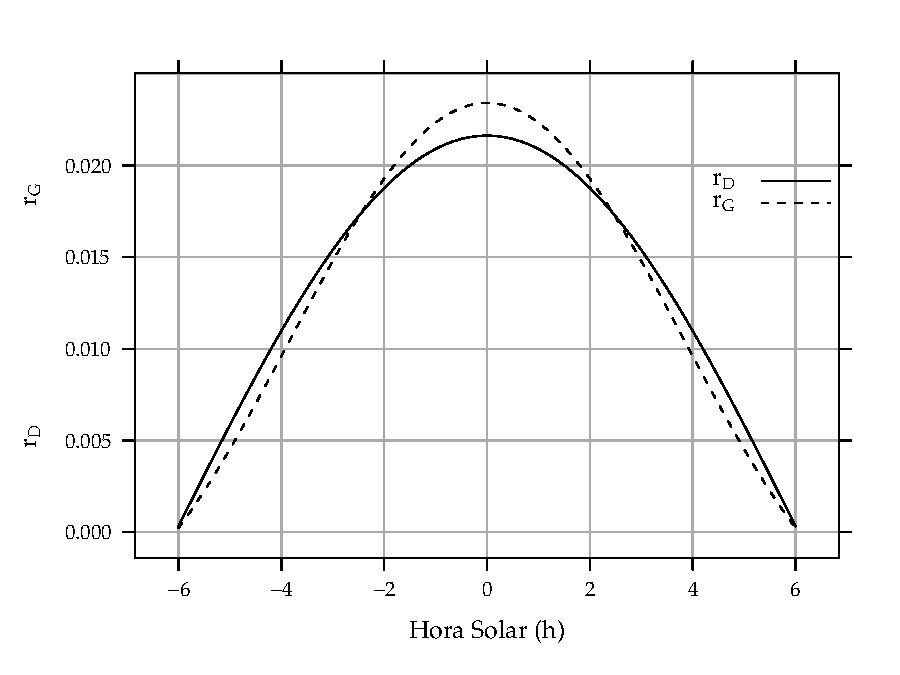
\includegraphics[scale=0.6]{../Figuras/RgRd}
\par\end{center}


\end{frame}
\begin{frame}
\frametitle{Estimación de Irradiancia a partir de Irradiación diaria}
\begin{description}
\item [{Calcular}] la irradiancia global y la irradiancia difusa en el
plano horizontal 

\begin{description}
\item [{2}] horas antes del mediodía del día 261 en un lugar con latitud$\phi=\ang{40}\mathrm{N}$
y con media mensual de irradiación global diaria horizontal $G_{d,m}(0)=\SI{2700}{\watthour\per\meter\squared}$.
\end{description}
\end{description}

\end{frame}
\subsection{Transformación al plano del generador}


\begin{frame}
\frametitle{Irradiancia Directa}

\begin{block}
{}

\[
B(\beta,\alpha)=B(0)\cdot\frac{\max(0,\cos(\theta_{s}))}{\cos(\theta_{zs})}\]


\end{block}

\end{frame}
\begin{frame}
\frametitle{Factor de visión para Difusa}

\begin{center}
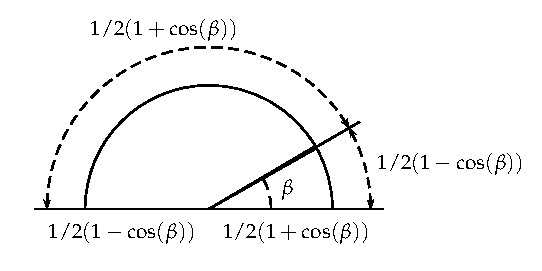
\includegraphics{../Figuras/AnguloVisionCielo}
\par\end{center}

\[
D(\beta,\alpha)=\intop_{\Omega}L(\theta_{z},\psi)\cdot\cos(\theta_{z}^{'})d\Omega\]



\end{frame}
\begin{frame}
\frametitle{Irradiancia Difusa isotrópica}
\begin{block}
{}

\[
L(\theta_{z},\psi)=cte.\]


\[
D(\beta,\alpha)=D(0)\cdot\frac{1+\cos(\beta)}{2}\]


\end{block}

\end{frame}
\begin{frame}
\frametitle{Irradiancia Difusa Anisotrópica}
\begin{block}
{}

\begin{eqnarray*}
D(\beta,\alpha) & = & D^{I}(\beta,\alpha)+D^{C}(\beta,\alpha)\\
D^{I}(\beta,\alpha) & = & D(0)\cdot(1-k_{1})\cdot\frac{1+\cos(\beta)}{2}\\
D^{C}(\beta,\alpha) & = & D(0)\cdot k_{1}\cdot\frac{\max(0,\cos(\theta_{s}))}{\cos(\theta_{zs})}\\
k_{1} & = & \frac{B(0)}{B_{0}(0)}\end{eqnarray*}


\end{block}

\end{frame}
\begin{frame}
\frametitle{Irradiancia de Albedo}
\begin{block}
{}

\[
R(\beta,\alpha)=\rho\cdot G(0)\cdot\frac{1-\cos(\beta)}{2}\]


\[
\rho=0.2\]


\end{block}

\end{frame}
\begin{frame}
\frametitle{Irradiancia sobre plano inclinado}
\begin{description}
\item [{Calcular}] la irradiancia difusa, directa, de albedo y global,
en 

\begin{description}
\item [{Un}] generador inclinado $\ang{30}$ y orientado al Sur, 2 horas
antes del mediodía del día 261 en un lugar con latitud $\phi=\ang{40}\mathrm{N}$
y con media mensual de irradiación global diaria horizontal $G_{d,m}(0)=\SI{2700}{\watthour\per\meter\squared}$.
\end{description}
\end{description}

\end{frame}
\subsection{Incertidumbre}


\begin{frame}[plain]
\frametitle{Variabilidad Interanual}

\begin{center}
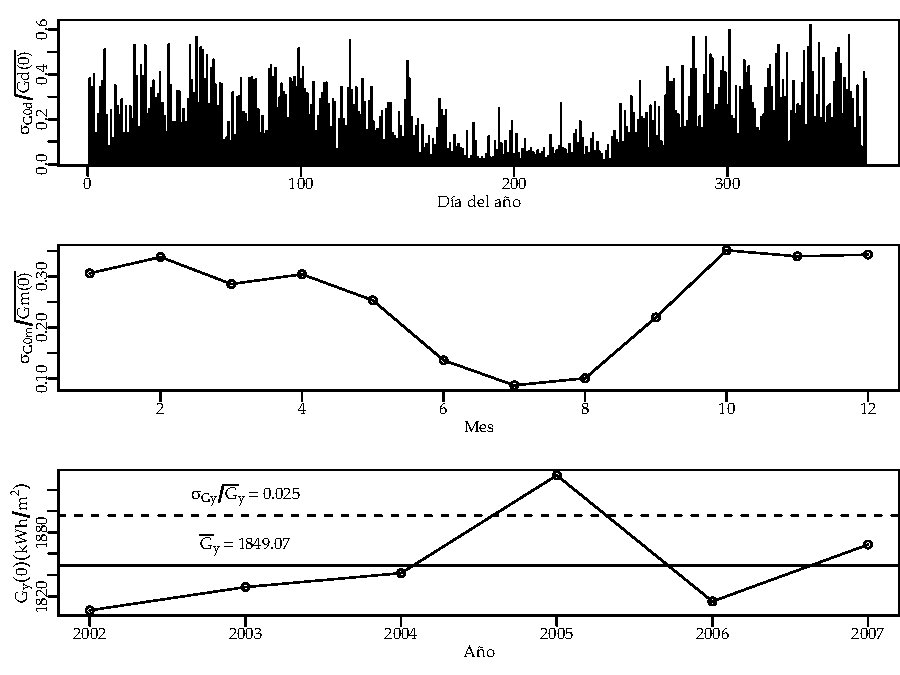
\includegraphics[scale=0.65]{../Figuras/VariabilidadRadiacionDiario}
\par\end{center}


\end{frame}
\begin{frame}
\frametitle{Incertidumbre}
\begin{itemize}
\item Predicción para un (día, mes, año) \emph{determinado}: 

\begin{itemize}
\item Intervalo de confianza del 95\% acotado por $1.96\cdot\sigma_{G}$
\end{itemize}
\item Predicción para un (día, mes, año) \emph{promedio (durante N años)}: 

\begin{itemize}
\item Intervalo de confianza del 95\% acotado por $1.96\cdot\sigma_{\overline{G}}$
\end{itemize}
\end{itemize}
\[
\sigma_{\overline{G}}=\frac{\sigma_{G}}{\sqrt{N}}\]



\end{frame}
\subsection{Pérdidas angulares y por suciedad}


\begin{frame}
\frametitle{Radiación directa}
\begin{block}
{}

\[
B_{ef}(\beta,\alpha)=B(\beta,\alpha)\cdot\left[\frac{T_{sucio}(0)}{T_{limpio}(0)}\right]\cdot (1-FT_{B}(\theta_{s}))\]


\end{block}

\end{frame}
\begin{frame}
\frametitle{Pérdidas angulares para radiación directa}

\begin{center}
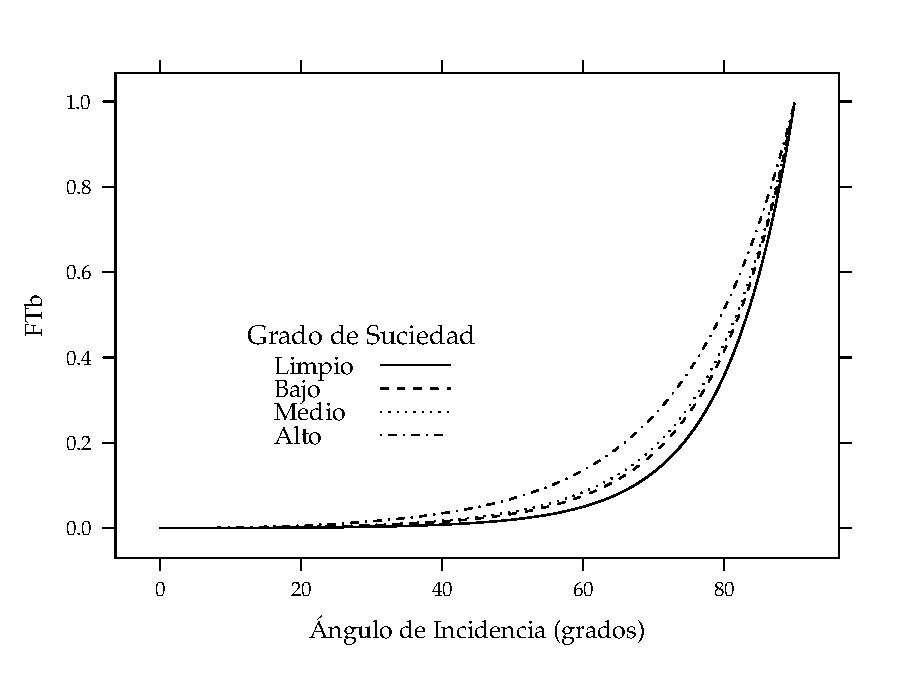
\includegraphics[scale=0.6]{../Figuras/Suciedad}
\par\end{center}


\end{frame}

\begin{frame}
\frametitle{Difusa y Albedo}
\begin{block}
{}

\begin{eqnarray*}
D_{ef}^{iso}(\beta,\alpha) & = & D^{iso}(\beta,\alpha)\cdot\left[\frac{T_{sucio}(0)}{T_{limpio}(0)}\right]\cdot(1-FT_{D}(\beta))\\
D_{ef}^{cir}(\beta,\alpha) & = & D^{cir}(\beta,\alpha)\cdot\left[\frac{T_{sucio}(0)}{T_{limpio}(0)}\right]\cdot(1-FT_{B}(\theta_{s}))\\
R_{ef}(\beta,\alpha) & = & R(\beta,\alpha)\cdot\left[\frac{T_{sucio}(0)}{T_{limpio}(0)}\right]\cdot(1-FT_{R}(\beta))\end{eqnarray*}


\end{block}

\end{frame}

\begin{frame}
\frametitle{Coeficientes}

\begin{center}
\begin{tabular}{cccc}
\toprule 
Grado de Suciedad & $\frac{T_{sucio}(0)}{T_{limpio}(0)}$ & $a_{r}$ & $c_{2}$\tabularnewline
\midrule 
Limpio & 1 & 0.17 & -0.069\tabularnewline
\midrule 
Bajo & 0.98 & 0.20 & -0.054\tabularnewline
\midrule 
Medio & 0.97 & 0.21 & -0.049\tabularnewline
\midrule 
Alto & 0.92 & 0.27 & -0.023\tabularnewline
\bottomrule
\end{tabular}
\par\end{center}


\end{frame}

\begin{frame}
\frametitle{Pérdidas anuales}

\begin{center}
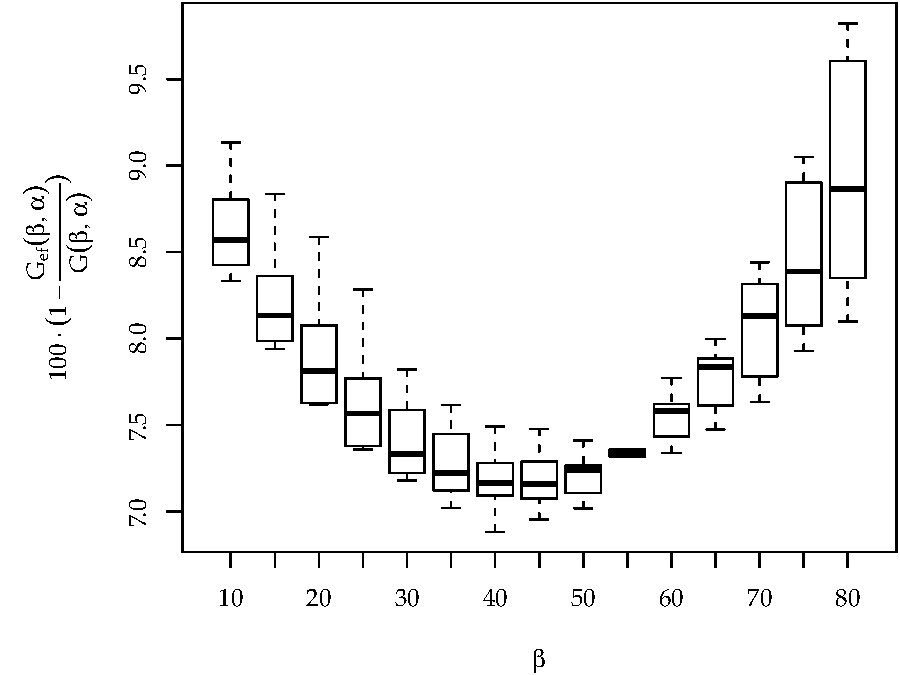
\includegraphics[scale=0.6]{../Figuras/GefVSG}
\par\end{center}


\end{frame}

\section{Radiación Efectiva según tipologías}

\begin{frame}[plain]
  \frametitle{Radiación en Sistema estático}

  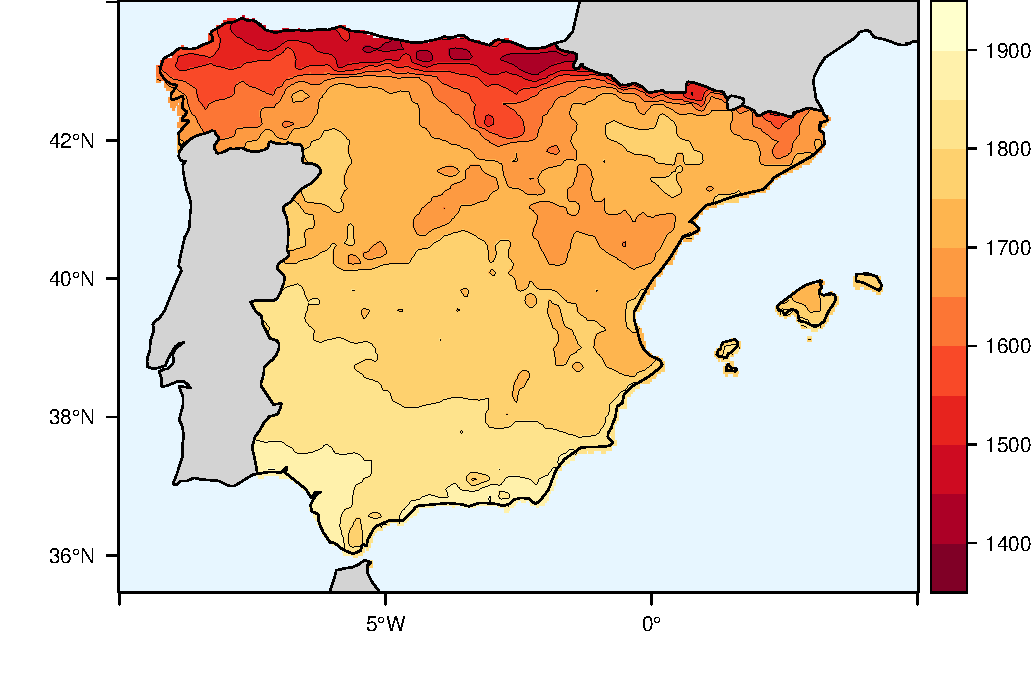
\includegraphics[width=\textwidth]{../Figuras/FixedKrig}
\end{frame}

\begin{frame}[plain]
  \frametitle{Radiación en Seguimiento Eje Horizontal}

  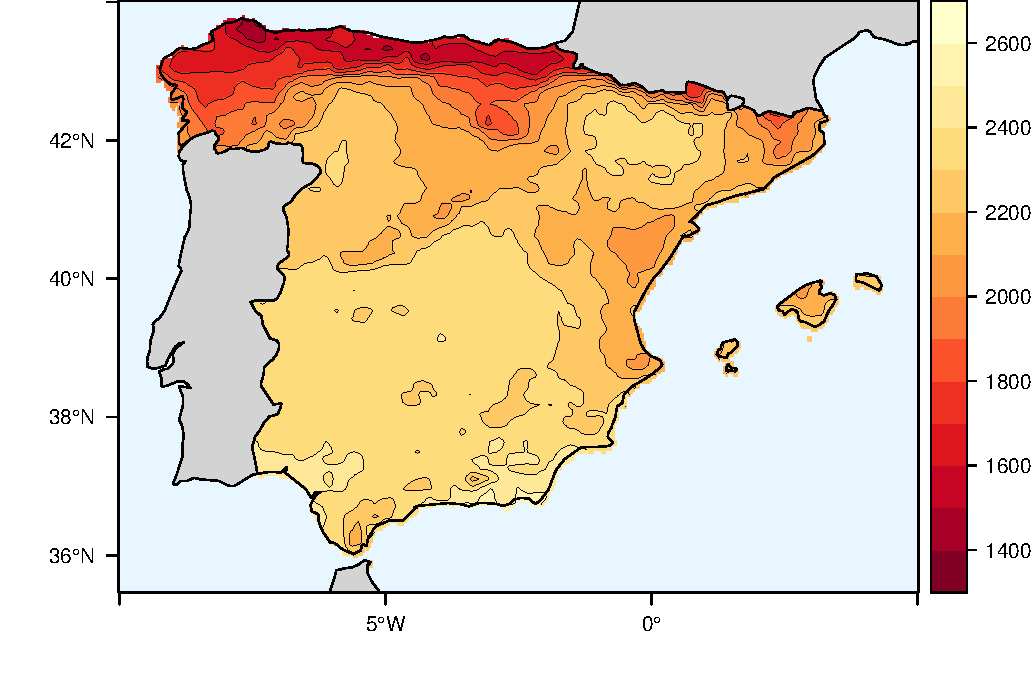
\includegraphics[width=\textwidth]{../Figuras/HorizKrig}

\end{frame}

\begin{frame}[plain]
  \frametitle{Radiación en Seguimiento Doble Eje}

  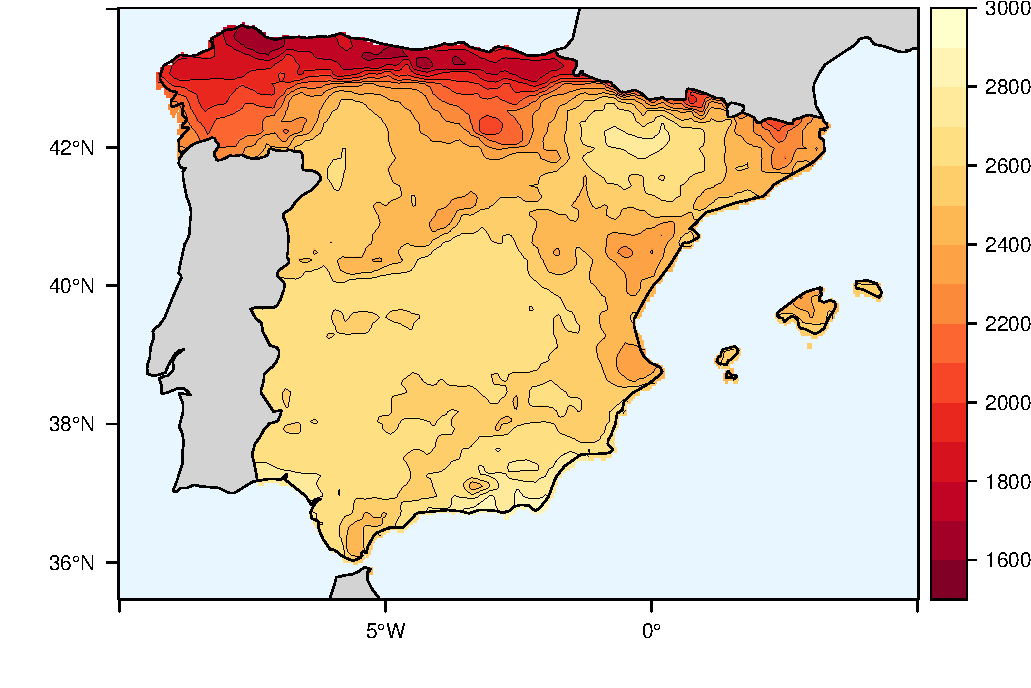
\includegraphics[width=\textwidth]{../Figuras/TwoKrig}

\end{frame}

\subsection{Comparación entre tipologías}

\begin{frame}[plain]
  \frametitle{Comparación Doble Eje-Estática}

  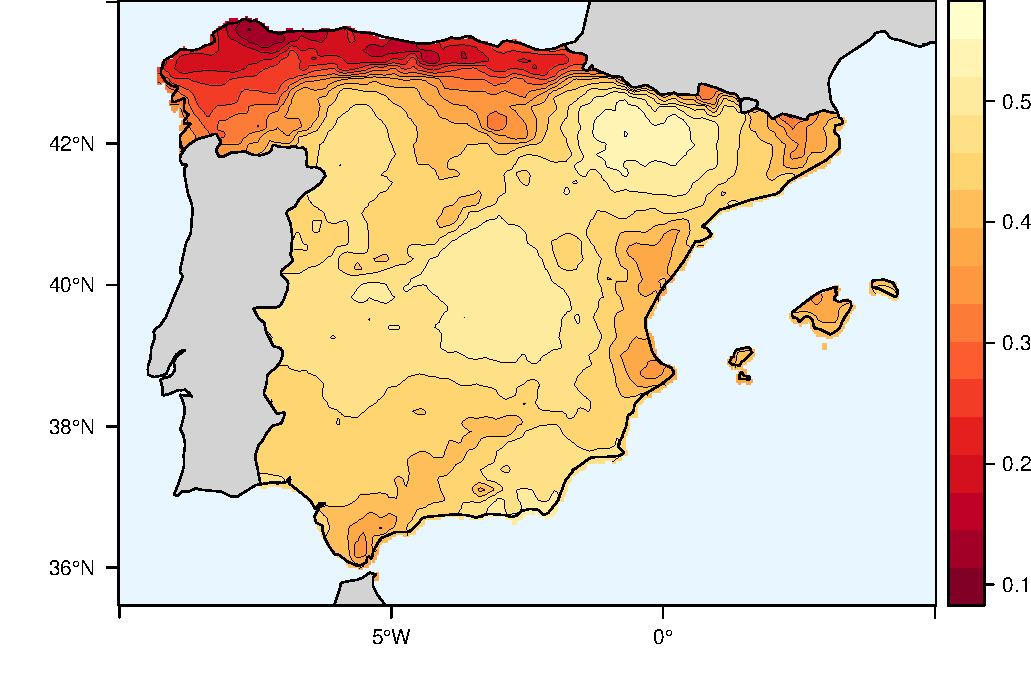
\includegraphics[width=\textwidth]{../Figuras/TwoFixed}


\end{frame}

\begin{frame}[plain]
  \frametitle{Comparación Doble Eje - Horizontal}

    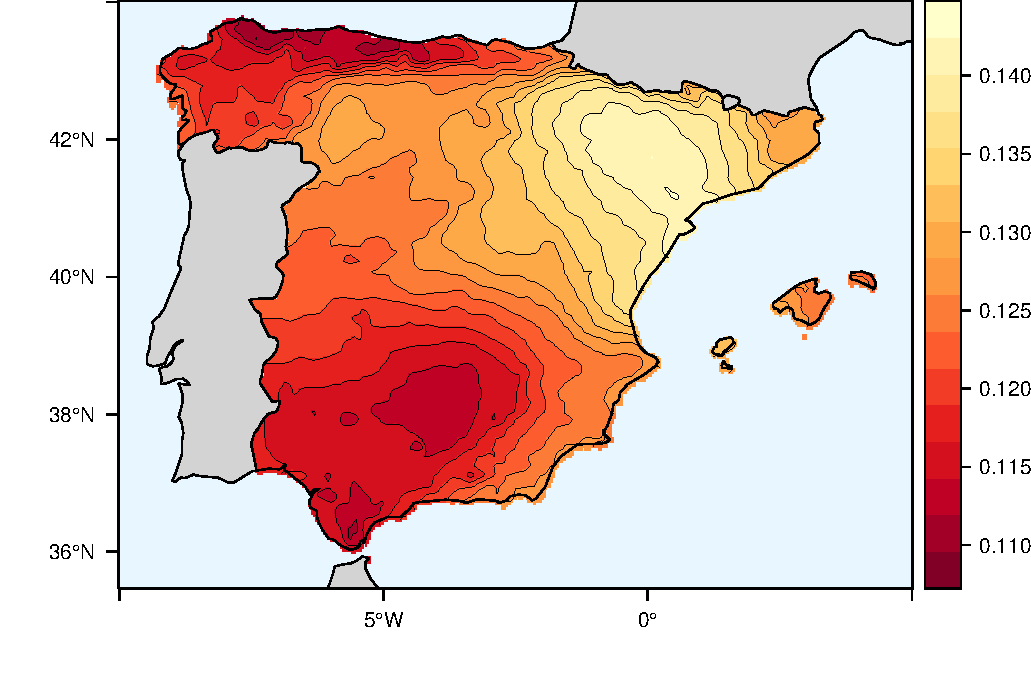
\includegraphics[width=\textwidth]{../Figuras/TwoHoriz}

\end{frame}

\begin{frame}[plain]
  \frametitle{Comparación Eje Horizontal - Estática}

    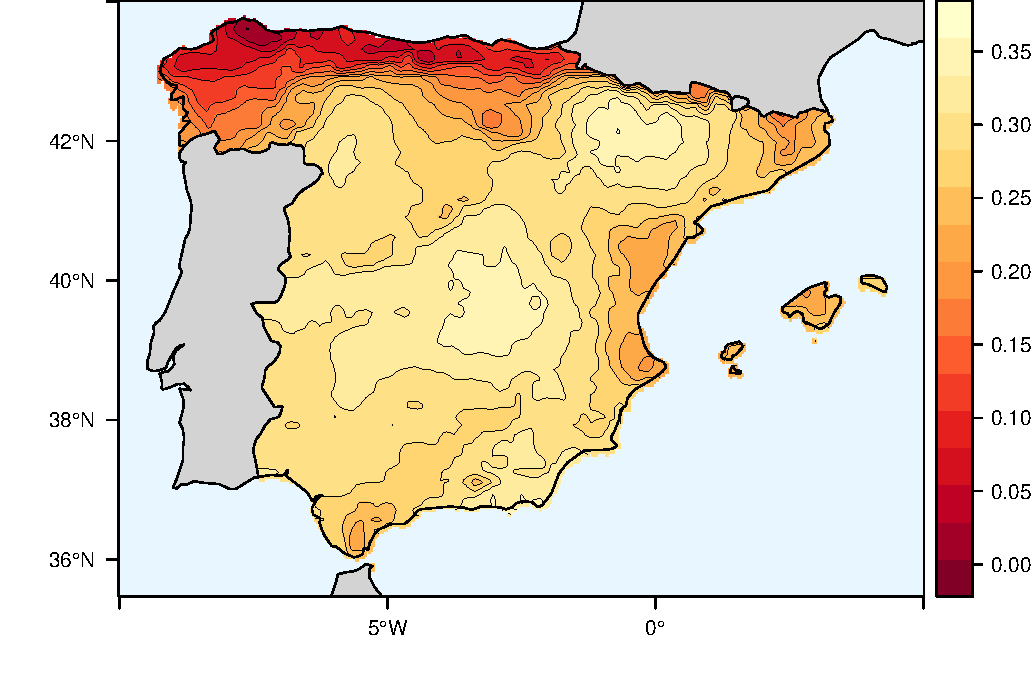
\includegraphics[width=\textwidth]{../Figuras/HorizFixed}

\end{frame}

\begin{frame}[plain]
  \frametitle{Comparación Eje Horizontal - Estática}
  \begin{columns}%{}


    \column{6cm}

    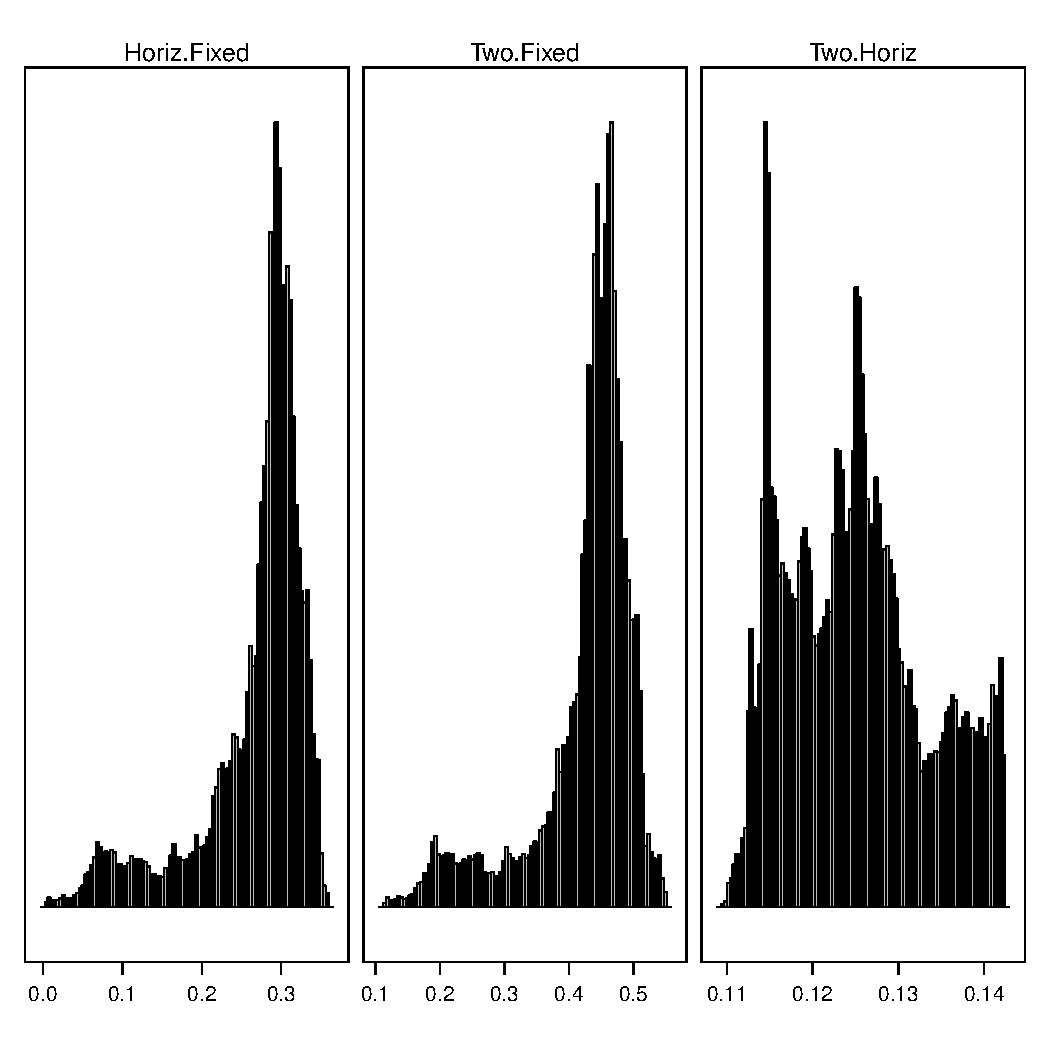
\includegraphics[width=6cm]{../Figuras/compSystems}

    \column{6cm}

    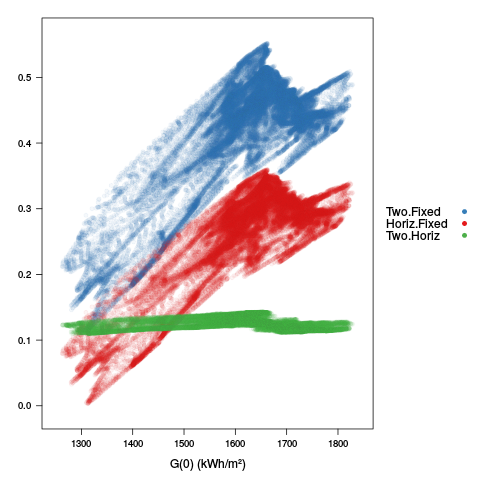
\includegraphics[width=6cm]{../Figuras/compSystemsG0}

  \end{columns}%{}
\end{frame}


\section{Aplicación a Sistemas estáticos}


\subsection{Ángulo de inclinación óptimo}


\begin{frame}
\frametitle{Inclinación Optima Estática}
\begin{block}
{}

\[
\left|\phi\right|-\beta\approx10\degree\]


\[
\beta_{opt}=3.7+0.69\cdot|\phi|\]


\end{block}

\end{frame}
\begin{frame}
\frametitle{Sensibilidad al desapuntamiento}

\begin{center}
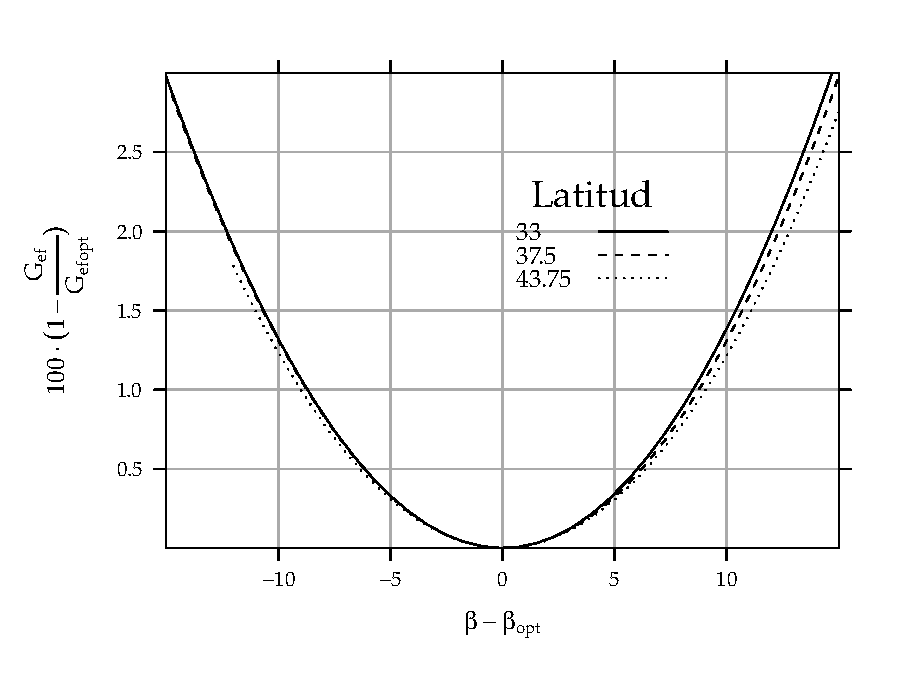
\includegraphics[scale=0.6]{../Figuras/PerdidasInclinacionOptima}
\par\end{center}


\end{frame}
\begin{frame}
\frametitle{Radiación para inclinación óptima}
\begin{block}
{}

\[
\frac{G_{d,a}(0)}{G_{d,a}(\beta_{opt})}=1-4.46\cdot10^{-4}\cdot\beta_{opt}-1.19\cdot10^{-4}\cdot\beta_{opt}^{2}\]


\end{block}

\end{frame}
\begin{frame}
\frametitle{Cálculo de Radiación Efectiva}
\begin{block}
{}

\begin{eqnarray*}
\frac{G_{efd,a}(\beta,\alpha)}{G_{d,a}(\beta_{opt})} & = & g_{1}\cdot(\beta-\beta_{opt})^{2}+g_{2}\cdot(\beta-\beta_{opt})+g_{3}\\
g_{i} & = & g_{i1}|\alpha|^{2}+g_{i2}|\alpha|+g_{i3}\end{eqnarray*}


\end{block}

\end{frame}
\begin{frame}
\frametitle{Cálculo para estática}

\begin{center}
\begin{tabular}{cccc}
\toprule
\textrm{$\frac{T_{sucio}(0)}{T_{limpio}(0)}=0.97$} & $i=1$ & $i=2$ & $i=3$\tabularnewline
\midrule 
$g_{1i}$ & $8\cdot10^{-9}$ & $3.8\cdot10^{-7}$ & $-1.218\cdot10^{-4}$\tabularnewline
\midrule 
$g_{2i}$ & $-4.27\cdot10^{-7}$ & $8.2\cdot10^{-6}$ & $2.892\cdot10^{-4}$\tabularnewline
\midrule 
$g_{3i}$ & $-2.5\cdot10^{-5}$ & $-1.034\cdot10^{-4}$ & $0.9314$\tabularnewline
\bottomrule
\end{tabular}
\par\end{center}


\end{frame}

\begin{frame}
\frametitle{Cálculo para estática}
\begin{description}
\item [{Calcular}] la irradiación anual efectiva que incide en 

\begin{description}
\item [{{\small Un}}] {\small generador orientado al Sur e inclinado $\ang{20}$
en un lugar con latitud $\ang{30}\mathrm{N}$ y una media anual de
la irradiación global diaria en el plano horizontal de $\SI{5250}{\watthour\per\meter\squared}$,
suponiendo una suciedad media.}{\small \par}
\end{description}
\item [{Calcular}] la irradiación anual efectiva que incide en 

\begin{description}
\item [{{\small Un}}] {\small generador desorientado $\ang{20}$del Sur
e inclinado $\ang{40}$ en un lugar con latitud $\ang{50}\mathrm{N}$
y una media anual de la irradiación global diaria en el plano horizontal
de $\SI{5250}{\watthour\per\meter\squared}$, suponiendo una suciedad
media.}{\small \par}
\end{description}
\end{description}

\end{frame}





\end{document}
